\chapter{Error Detection and Correction Codes to Protect an In-Core DIFT against FIAs}
\chaptermark{Error Detection and Correction codes to protect an In-Core DIFT against FIAs}
\label{chapter:countermeasures}
\minitoc

%%%%%%%%%%%%%%%%%%%%%%%%%%%%%%%%%%%%%%%%%%%%%%%%%%%%%%%%%%%%%%%%%%%%%%%%%%%%%%%%%%%%%%%%%%%%%%%
\section{Introduction}
Previous chapters have shown that the D-RI5CY's DIFT security mechanism is vulnerable to FIAs, mainly due to single-bit flips. This D-RI5CY essentially uses single-bit registers, as it relies on 1-bit tags.

In this chapter, we present three countermeasures in order to protect the DIFT against FIAs.
The first countermeasure implemented to detect and prevent the use of corrupted data is simple parity. We selected the simple parity code as the error detection countermeasure because of its suitability and limited overhead. However, parity codes are limited in that they can only detect, but not correct, single-bit errors.
The second countermeasure is implemented to detect any single-bit errors that may occur, but also to correct them without time overhead. With this countermeasure, we want to correct to the nearest cycle so that the fault cannot propagate and show to a potential attacker that the fault he injected had no effect on the system.
The third countermeasure is called SECDED for Single Error Correction, Double Error Detection. This protection is a Hamming Code extended with a single parity bit to allow the detection of double-bit errors while being able to correct single-bit errors.
This chapter presents the work done during a 4-month research stay, funded by the \textit{Collège Doctoral de Bretagne}, \textit{GDR ISIS (CNRS)}, and the \textit{Université Bretagne Sud}, within the \textit{ALaRI} laboratory (\textit{Advanced Learning and Research Institute}) in the \textit{Università della Svizzera Italiana} in Lugano, Switzerland.
This work has been published in ISVLSI 2024~\cite{PRLG-24-isvlsi}.

The first section presents the different considered fault models. Then, the second section presents simple parity and details its implementation. Afterwards, the third section presents Hamming Code principles, with a simple example, and details our implementation. The fourth section presents SECDED with an example and gives an overview on our implementation. Finally, we discuss these countermeasures and compare them.

%%%%%%%%%%%%%%%%%%%%%%%%%%%%%%%%%%%%%%%%%%%%%%%%%%%%%%%%%%%%%%%%%%%%%%%%%%%%%%%%%%%%%%%%%%%%%%%
\section{Fault models considered in this chapter}
In Chapter~\ref{chapter:dift_assessment}, we assessed the D-RI5CY design by considering \textit{single bit-flip in one register at a given clock cycle}, \textit{bit reset}, and \textit{bit set} fault models. The conclusion of this chapter was that the D-RI5CY is vulnerable mostly to single bit-flip, due to the fact that this DIFT design is mostly built around 1-bit registers for tag propagation.

In this chapter, we consider an attacker able to inject faults into DIFT-related registers, leading to single bit-flips at any position of the targeted register. To reach this objective, any DIFT-related register maintaining 1-bit tag value, driving the tag propagation or the tag update process or maintaining the security policy configuration can be targeted. Studies presented in~\cite{ZDCRT-12-dcis,CLFT-14-cosade} have shown that such precise single bit-flip attacks targeting registers can be performed using, for example, laser shots. We also consider an attacker able to inject a \textit{single bit-flip in two registers at two distinct clock cycles}, with a minimum delay of one clock cycle. Nowadays, more and more platforms exist to perform multi-bits faults on different targets~\cite{alphanov-doubleLFI,alphanov-fourLFI}. These platforms are helping to spread the use of this type of attack, thus we should also be forging our protection around these kinds of threats.

\begin{table}
    \centering
    \small
    \caption{D-RI5CY Registers Details List}
    \label{tab:driscy_register_info}
    \begin{tabular}{rlcc}
        \toprule
        Register Name                   & Module                                            & Size & Group \\
        \midrule
        pc\_id\_o\_tag                  & \textcolor{red}{Instruction Fetch Stage}          & 1    & Gr5   \\
        pc\_if\_o\_tag                  & \textcolor{red}{Instruction Fetch Stage}          & 1    & Gr5   \\\hdashline
        alu\_operand\_a\_ex\_o\_tag     & \textcolor{blue}{Instruction Decode Stage}        & 1    & Gr5   \\
        alu\_operand\_b\_ex\_o\_tag     & \textcolor{blue}{Instruction Decode Stage}        & 1    & Gr5   \\
        alu\_operand\_c\_ex\_o\_tag     & \textcolor{blue}{Instruction Decode Stage}        & 1    & Gr5   \\
        alu\_operator\_o\_mode          & \textcolor{blue}{Instruction Decode Stage}        & 2    & Gr5   \\
        check\_d\_o\_tag                & \textcolor{blue}{Instruction Decode Stage}        & 1    & Gr5   \\
        check\_s1\_o\_tag               & \textcolor{blue}{Instruction Decode Stage}        & 1    & Gr5   \\
        check\_s2\_o\_tag               & \textcolor{blue}{Instruction Decode Stage}        & 1    & Gr5   \\
        is\_store\_post\_o\_tag         & \textcolor{blue}{Instruction Decode Stage}        & 1    & Gr5   \\
        memory\_set\_o\_tag             & \textcolor{blue}{Instruction Decode Stage}        & 1    & Gr5   \\
        regfile\_alu\_waddr\_ex\_o\_tag & \textcolor{blue}{Instruction Decode Stage}        & 5    & Gr4   \\
        register\_set\_o\_tag           & \textcolor{blue}{Instruction Decode Stage}        & 1    & Gr5   \\
        store\_dest\_addr\_ex\_o\_tag   & \textcolor{blue}{Instruction Decode Stage}        & 1    & Gr5   \\
        store\_source\_ex\_o\_tag       & \textcolor{blue}{Instruction Decode Stage}        & 1    & Gr5   \\
        use\_store\_ops\_ex\_o          & \textcolor{blue}{Instruction Decode Stage}        & 1    & Gr5   \\\hdashline
        rf\_reg[0]                      & \textcolor{LimeGreen}{Register File Tag}          & 1    & Gr3   \\
        rf\_reg[1]                      & \textcolor{LimeGreen}{Register File Tag}          & 1    & Gr3   \\
        rf\_reg[2]                      & \textcolor{LimeGreen}{Register File Tag}          & 1    & Gr3   \\
        \ldots                      & \textcolor{LimeGreen}{Register File Tag}          & \ldots    & Gr3   \\
        rf\_reg[30]                     & \textcolor{LimeGreen}{Register File Tag}          & 1    & Gr3   \\
        rf\_reg[31]                     & \textcolor{LimeGreen}{Register File Tag}          & 1    & Gr3   \\\hdashline
        rs1\_o\_tag                     & \textcolor{DarkOrange}{Execute Stage}             & 1    & Gr5   \\\hdashline
        tcr\_q                          & \textcolor{DarkRed}{Control and Status Registers} & 32   & Gr1   \\
        tpr\_q                          & \textcolor{DarkRed}{Control and Status Registers} & 32   & Gr2   \\\hdashline
        data\_type\_q\_tag              & \textcolor{magenta}{Load/Store Unit}              & 2    & Gr5   \\
        data\_we\_q\_tag                & \textcolor{magenta}{Load/Store Unit}              & 1    & Gr5   \\
        rdata\_offset\_q\_tag           & \textcolor{magenta}{Load/Store Unit}              & 2    & Gr5   \\
        rdata\_q\_tag                   & \textcolor{magenta}{Load/Store Unit}              & 4    & Gr5   \\
        \bottomrule
    \end{tabular}
\end{table}
    

%%%%%%%%%%%%%%%%%%%%%%%%%%%%%%%%%%%%%%%%%%%%%%%%%%%%%%%%%%%%%%%%%%%%%%%%%%%%%%%%%%%%%%%%%%%%%%%
\section{Simple Parity}
\label{chapter:simpleparity}

Parity codes represent one of the simplest and most fundamental methods for error detection in digital communication systems. Utilised across a wide range of applications, parity codes help to ensure data integrity by adding a single parity bit to a block of data. This bit acts as a basic error-detection mechanism, enabling the identification of single-bit errors during transmission. Parity codes are commonly classified into two types: even parity and odd parity. In an even parity system, the parity bit is set such that the total number of 1s in the data block, including the parity bit, is even. Conversely, in an odd parity system, the parity bit is adjusted so that the number of \texttt{1} is odd.

%%%%%%%%%%%%%%%%%%%%%%%%%%%%%%
\subsection{Simple parity in a nutshell}
The key advantage of parity codes lies in their simplicity and low overhead. A single parity bit, added to each data block, is sufficient to detect any single-bit error in the block. This one bit stores the parity of the initial message. Figure~\ref{fig:simpleparity_functionning} shows how the data, in blue, and the parity bit, in red, are associated to form an encoded data.

\begin{figure}[ht]
    \centering
    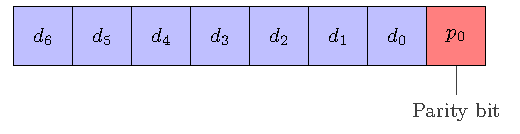
\includegraphics[page=1]{c5_countermeasures_dift/img/simple_parity.pdf}
    \caption{Simple Parity -- functioning}
    \label{fig:simpleparity_functionning}
\end{figure}

Equation~\ref{equat:simpleparity} shows how the parity bit is computed. Each bit of the initial message is XOR'd to calculate parity.

\begin{equation} \label{equat:simpleparity}
    \begin{split}
        p_{0} &= d_{0} \oplus d_{1} \oplus d_{2} \oplus d_{3} \oplus d_{4} \oplus d_{5} \oplus d_{6}
    \end{split}
\end{equation}

Figures~\ref{fig:simpleparity_example_1} and \ref{fig:simpleparity_example_2} show an example of a message with its parity bit. The message is \texttt{0b1001101}. Hence, as there is an even number of '\texttt{1}', the parity bit is set to '\texttt{0}'.

\begin{figure}[ht]
    \centering
    \begin{subfigure}[b]{0.49\textwidth}
        \includegraphics[width=\textwidth, page=2]{c5_countermeasures_dift/img/simple_parity.pdf}
        \caption{Initial message}
        \label{fig:simpleparity_example_1}
    \end{subfigure}
    \hfill
    \begin{subfigure}[b]{0.49\textwidth}
        \includegraphics[width=\textwidth, page=3]{c5_countermeasures_dift/img/simple_parity.pdf}
        \caption{Message with its parity bit}
        \label{fig:simpleparity_example_2}
    \end{subfigure}
    \hfill
    \begin{subfigure}[b]{0.49\textwidth}
        \includegraphics[width=\textwidth, page=4]{c5_countermeasures_dift/img/simple_parity.pdf}
        \caption{Single-bit fault inside the message}
        \label{fig:simpleparity_faulted_example_3}
    \end{subfigure}
    \hfill
    \begin{subfigure}[b]{0.49\textwidth}
        \includegraphics[width=\textwidth, page=5]{c5_countermeasures_dift/img/simple_parity.pdf}
        \caption{Two single-bit faults inside the message}
        \label{fig:simpleparity_faulted_example_4}
    \end{subfigure}
    \caption{Example of a simple parity calculation and its fault detection capacity}
    \label{fig:simpleparity_example}
\end{figure}

Figures~\ref{fig:simpleparity_faulted_example_3} and \ref{fig:simpleparity_faulted_example_4} present, respectively, two examples of when a fault occurs and when two faults happen.
In the first example, Figure~\ref{fig:simpleparity_faulted_example_3}, the bit $d_2$ (from Figure~\ref{fig:simpleparity_functionning}), in red, is faulted. As the faulted message is \texttt{0b1001001}, it means that the new calculated parity bit value should be \texttt{1}. Hence, the fault will be detected as the parity bit differs from the original computed message (Figure~\ref{fig:simpleparity_example_2}).
In the second case, two faults happen in the message at bits $d_2$ and $d_5$ (from Figure~\ref{fig:simpleparity_functionning}). So, the faulted message is \texttt{0b1101001}, then, when the new parity bit is calculated, the parity bit value will not change as there is still an even number of \texttt{1} compared to the initial message. This shows the limitation of this error detection code.

%%%%%%%%%%%%%%%%%%%%%%%%%%%%%%
\subsection{Implementation: Minimisation of redundancy bits}

In order to implement simple parity, we decided, in a first approach, to optimise the number of parity bits. We had different choices, but we decided to form five groups. These groups are composed of one or more register according to their criticality. Table~\ref{tab:driscy_register_info} presents all 55 registers of the D-RI5CY mechanism with their size (in number of bits) and the group in which they are associated with. Each colour represents a different HDL module.
Firstly, the two registers that contain the security policy, TCR and TPR, are highly critical. As a result, we have chosen to form a separate group for each of them. Although these registers are 32 bits long, only 22 bits are fully utilised in the current implementation, making bits 22 to 31 unnecessary. Therefore, we have decided not to protect these unused bits or include them in parity calculations.
Secondly, the third logical group consists of keeping the 32 registers of the register file tag together. Since these registers are already grouped, it makes sense to maintain this grouping.
This leaves us with one 5-bit register, sixteen 1-bit registers, three 2-bit registers, and one 4-bit register. The 5-bit register is used to store the tag destination address, which is critical. As such, we have decided to create a dedicated group for it. The remaining 20 registers, which total 26 bits, are combined into a fifth group.
Table~\ref{tab:sp_group} shows the five groups formed to implement the protection for 107 bits in total. One parity bit protects each group.

\begin{table}[t]
    \centering
    \footnotesize
    \caption{DIFT-related protected registers -- simple parity}
    \label{tab:sp_group}
    \begin{tabular}{@{}ccccc@{}}
        \toprule
                & Protected register                                                                                & \begin{tabular}[c]{@{}c@{}}Number of\\ bits\end{tabular} & \begin{tabular}[c]{@{}c@{}}Number of\\ protected bits\end{tabular} & \begin{tabular}[c]{@{}c@{}}Number of\\ parity bits\end{tabular} \\ \midrule
        Group 1 & TCR                                                                                               & 32                                                       & 22                                                                 & 1                                                               \\
        Group 2 & TPR                                                                                               & 32                                                       & 22                                                                 & 1                                                               \\
        Group 3 & Register File (Tag)                                                                               & 32                                                       & 32                                                                 & 1                                                               \\
        Group 4 & Tag destination address                                                                           & 5                                                        & 5                                                                  & 1                                                               \\
        Group 5 & \begin{tabular}[c]{@{}c@{}}16×1-bit registers\\ 3×2-bit registers\\ 1×4-bit register\end{tabular} & 26                                                       & 26                                                                 & 1                                                               \\ \midrule
        Total   &                                                                                                   & 127                                                      & 107                                                                & 5                                                               \\
        \bottomrule
    \end{tabular}
\end{table}

Figure~\ref{fig:implementation_sp} presents our proposed implementation for the simple parity. This implementation is straightforward. To protect a register (shown in blue), the input is directed simultaneously to both the protected register and an encoder (in green). The encoder calculates the parity using combinatorial logic, storing the resulting parity bit in a separate register, depicted in salmon-red in the figure. The parity bit is stored in this register during the same cycle as the input value is stored in the protected register. Subsequently, the decoder computes the parity of the protected register and compares it with the parity bit stored in the parity bit register. If a difference is detected, it indicates the injection of a fault, which causes an alert signal to be raised.

\begin{figure}[ht]
    \centering
    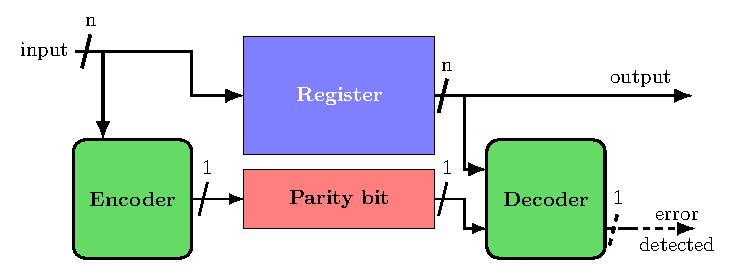
\includegraphics[page=1]{c5_countermeasures_dift/img/archi_contremesures.pdf}
    \caption{Implementation of simple parity}
    \label{fig:implementation_sp}
\end{figure}

%%%%%%%%%%%%%%%%%%%%%%%%%%%%%%%%%%%%%%%%%%%%%%%%%%%%%%%%%%%%%%%%%%%%%%%%%%%%%%%%%%%%%%%%%%%%%%%
\section{Hamming Codes}
\label{chapter:hammingcode}

In digital communication and error correction theory, Hamming Codes represent a pioneering development in ensuring data integrity during transmission over unreliable channels. Developed by Richard Hamming in 1950~\cite{H-50-bstj}, this class of error-correcting codes is designed to detect and correct single-bit errors and detect, without the correction part, two-bit errors. The Hamming Code is a linear block code that enhances data transmission reliability by introducing redundancy in a structured manner.

The importance of Hamming Codes lies not only in their ability to maintain the integrity of data but also in their efficiency relative to other early error correction schemes. As such, Hamming Codes have found wide application in areas where high data accuracy is required, such as computer memory systems, telecommunications, and satellite communication. Despite the emergence of more sophisticated error-correcting codes in modern systems, the simplicity and effectiveness of Hamming Codes make them a foundational topic in the study of error correction algorithms.

%%%%%%%%%%%%%%%%%%%%%%%%%%%%%%
\subsection{Hamming Code in a nutshell}

\begin{figure}[ht]
    \centering
    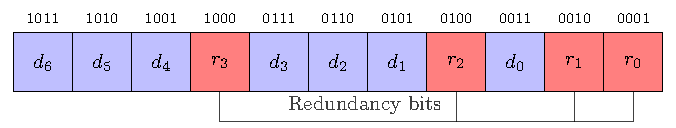
\includegraphics[page=1]{c5_countermeasures_dift/img/hamming_bit.pdf}
    \caption{Hamming Code (11,7) -- functioning}
    \label{fig:hamming_functionning}
\end{figure}

The fundamental principle behind the Hamming Code is the strategic insertion of $r$ redundancy bits at specific positions within a data block of $d$ bits, such that \(2^r \geqslant d + r + 1\).
These parity bits are used to perform checks on subsets of data bits, allowing the receiver to identify and, in certain cases, correct erroneous bits. The placement and calculation of the parity bits follow a binary positional system (1, 2, 4, 8, 16, \ldots), which forms the core of the error detection and correction mechanism. For example, for an 8-bit word it needs four redundancy bits while for a 64-bit word, it needs only 7 redundancy bits. By positioning the redundancy bits at the indexes of powers of two, it is then possible to correct an error if one is detected. Thus, for example, Hamming Code (11,7) owns seven bits of data ($d_{0}-d_{6}$) and four redundancy bits ($r_{0}-r_{3}$). Data bits and redundancy bits are placed according to Figure~\ref{fig:hamming_functionning}. The most common Hamming Code is the (7,4), which uses four data bits and three redundancy bits.
For the Hamming Code (11,7) (Figure~\ref{fig:hamming_functionning}), redundancy bits are computed according to Equation~\ref{equat:hamming_encoder}. This equation calculation is also represented in Figure~\ref{fig:hamming_code_example}. For example, if the initial message to be sent is \texttt{0b1001101} in binary, the redundancy bit $r_0$ will be computed as $r_0 = d_{0} \oplus d_{1} \oplus d_{3} \oplus d_{4} \oplus d_{6}$. Thus, $r_0$ will be equals to \texttt{1} as depicted in Figure~\ref{fig:hamming_code_example_2}. It is worth noting that this code is not fully used, because with four redundancy bits, Hamming Code is able to protect up to eleven data bits to form Hamming Code (15,11).

\begin{equation} \label{equat:hamming_encoder}
    \begin{split}
        r_{0} = d_{0} \oplus d_{1} \oplus d_{3} \oplus d_{4} \oplus d_{6} \\
        r_{1} = d_{0} \oplus d_{2} \oplus d_{3} \oplus d_{5} \oplus d_{6} \\
        r_{2} = d_{1} \oplus d_{2} \oplus d_{3} \\
        r_{3} = d_{4} \oplus d_{5} \oplus d_{6}
    \end{split}
\end{equation}

\begin{figure}[ht]
    \centering
    \begin{subfigure}[b]{0.49\textwidth}
        \includegraphics[width=\textwidth, page=2]{c5_countermeasures_dift/img/hamming_bit.pdf}
        \caption{Initial message}
        \label{fig:hamming_code_example_1}
    \end{subfigure}
    \hfill
    \begin{subfigure}[b]{0.49\textwidth}
        \includegraphics[width=\textwidth, page=4]{c5_countermeasures_dift/img/hamming_bit.pdf}
        \caption{Calculation of redundancy bit $r_0$}
        \label{fig:hamming_code_example_2}
    \end{subfigure}
    \hfill
    \begin{subfigure}[b]{0.49\textwidth}
        \includegraphics[width=\textwidth, page=6]{c5_countermeasures_dift/img/hamming_bit.pdf}
        \caption{Calculation of redundancy bit $r_1$}
        \label{fig:hamming_code_example_3}
    \end{subfigure}
    \hfill
    \begin{subfigure}[b]{0.49\textwidth}
        \includegraphics[width=\textwidth, page=8]{c5_countermeasures_dift/img/hamming_bit.pdf}
        \caption{Calculation of redundancy bit $r_2$}
        \label{fig:hamming_code_example_4}
    \end{subfigure}
    \hfill
    \begin{subfigure}[b]{0.49\textwidth}
        \includegraphics[width=\textwidth, page=10]{c5_countermeasures_dift/img/hamming_bit.pdf}
        \caption{Calculation of redundancy bit $r_3$}
        \label{fig:hamming_code_example_5}
    \end{subfigure}
    \caption{Hamming Code (11,7) redundancy bits calculations}
    \label{fig:hamming_code_example}
\end{figure}

\begin{equation} \label{equat:hamming_decoder}
    \begin{split}
        nr_{0} = r_{0} \oplus d_{0} \oplus d_{1} \oplus d_{3} \oplus d_{4} \oplus d_{6} = 1 \oplus 1 \oplus 0 \oplus 0 \oplus 0 \oplus 1    = 1 \\
        nr_{1} = r_{1} \oplus d_{0} \oplus d_{2} \oplus d_{3} \oplus d_{5} \oplus d_{6} = 0 \oplus 1 \oplus 1 \oplus 0 \oplus 0 \oplus 1    = 1 \\
        nr_{2} = r_{2} \oplus d_{1} \oplus d_{2} \oplus d_{3}                           = 0 \oplus 0 \oplus 1 \oplus 0                      = 1 \\
        nr_{3} = r_{3} \oplus d_{4} \oplus d_{5} \oplus d_{6}                           = 1 \oplus 0 \oplus 0 \oplus 1                      = 0
    \end{split}
\end{equation}

Figure~\ref{fig:hamming_code_faulted} presents an example of the detection and correction of an error. Figure~\ref{fig:hamming_code_faulted_1} depicts the message sent \texttt{0b10011100101} (1253 in decimal). A fault occurs during the transmission in the bit $d_3$ (Figure~\ref{fig:hamming_code_faulted_2} at position \texttt{0111}). The received message is \texttt{0b10010100101} (1189 in decimal).
During the verification of the redundancy bits. The equation~\ref{equat:hamming_decoder} shows how the new redundancy bits are calculated from the received redundancy and data bits. The association of these new redundancy bits ($nr_{0}-nr_{3}$) is call the syndrome. This syndrome represents the position of the faulted bit and needs to be read backward from $nr_3$ to $nr_0$. As shown in Equation~\ref{equat:hamming_decoder}, the syndrome equals \texttt{0b0111}. This is the correct position of the fault that happened in Figure~\ref{fig:hamming_code_faulted_2}. The same sequence is realised if a fault happens in a redundancy bit. This can be explained as each data bit is checked by at least two redundancy bits, while a redundancy bit is checked only by itself during the decoding phase.

\begin{figure}[ht]
    \centering
    \begin{subfigure}[b]{0.49\textwidth}
        \includegraphics[width=\textwidth, page=11]{c5_countermeasures_dift/img/hamming_bit.pdf}
        \caption{Initial message}
        \label{fig:hamming_code_faulted_1}
    \end{subfigure}
    \hfill
    \begin{subfigure}[b]{0.49\textwidth}
        \includegraphics[width=\textwidth, page=12]{c5_countermeasures_dift/img/hamming_bit.pdf}
        \caption{Injection of a fault in bit $d_3$}
        \label{fig:hamming_code_faulted_2}
    \end{subfigure}
    \hfill
    \begin{subfigure}[b]{0.49\textwidth}
        \includegraphics[width=\textwidth, page=13]{c5_countermeasures_dift/img/hamming_bit.pdf}
        \caption{Calculation of redundancy bit $r_0$}
        \label{fig:hamming_code_faulted_3}
    \end{subfigure}
    \hfill
    \begin{subfigure}[b]{0.49\textwidth}
        \includegraphics[width=\textwidth, page=14]{c5_countermeasures_dift/img/hamming_bit.pdf}
        \caption{Calculation of redundancy bit $r_1$}
        \label{fig:hamming_code_faulted_4}
    \end{subfigure}
    \hfill
    \begin{subfigure}[b]{0.49\textwidth}
        \includegraphics[width=\textwidth, page=15]{c5_countermeasures_dift/img/hamming_bit.pdf}
        \caption{Calculation of redundancy bit $r_2$}
        \label{fig:hamming_code_faulted_5}
    \end{subfigure}
    \hfill
    \begin{subfigure}[b]{0.49\textwidth}
        \includegraphics[width=\textwidth, page=16]{c5_countermeasures_dift/img/hamming_bit.pdf}
        \caption{Calculation of redundancy bit $r_3$}
        \label{fig:hamming_code_faulted_6}
    \end{subfigure}
    \caption{Example of a faulted message with Hamming Code (11,7)}
    \label{fig:hamming_code_faulted}
\end{figure}

%%%%%%%%%%%%%%%%%%%%%%%%%%%%%%
\subsection{Implementation: Minimisation of redundancy bits}

In order to implement Hamming Code, we used the same idea as the previous countermeasure: minimisation of redundancy bits. We used the same five groups as depicted in Table~\ref{tab:hammingcode_group}. As we only protect 22 bits of the 32 bits from TCR and TPR registers, we only need 5 bits of redundancy, instead of 6 bits.

\begin{table}[t]
    \centering
    \footnotesize
    \caption{DIFT-related protected registers -- Hamming Code}
    \label{tab:hammingcode_group}
    \begin{tabular}{@{}ccccc@{}}
        \toprule
                & Protected register                                                                                & \begin{tabular}[c]{@{}c@{}}Number of\\ bits\end{tabular} & \begin{tabular}[c]{@{}c@{}}Number of\\ protected bits\end{tabular} & \begin{tabular}[c]{@{}c@{}}Number of\\ redundancy bits\end{tabular} \\ \midrule
        Group 1 & TCR                                                                                               & 32                                                       & 22  & 5                                                                                                               \\
        Group 2 & TPR                                                                                               & 32                                                       & 22  & 5                                                                                                               \\
        Group 3 & Register File (Tag)                                                                               & 32                                                       & 32  & 6                                                                                                               \\
        Group 4 & Tag destination address                                                                           & 5                                                        & 5   & 4                                                                                                               \\
        Group 5 & \begin{tabular}[c]{@{}c@{}}16×1-bit registers\\ 3×2-bit registers\\ 1×4-bit register\end{tabular} & 26                                                       & 26  & 5                                                                                                               \\ \midrule
        Total   &                                                                                                   & 127                                                      & 107 & 25                                                                                                              \\
        \bottomrule
    \end{tabular}
\end{table}

Figure~\ref{fig:implementation_hc_1} presents the proposed implementation for Hamming Code. We do not integrate control signals for clarity. This implementation is straightforward. In order to protect a register or multiples independent registers, we choose to send the input(s) directly to both the protected register(s) (shown in blue) and an encoder. The encoder calculates the different redundancy bits using combinatorial logic, storing the resulting redundancy bits in a separate register, depicted in red in the figure. The redundancy bits are stored in this register at the same cycle as the input(s) value is (are) stored in the protected register(s). Subsequently, the decoder computes the parity of the protected register and compares it with the redundancy bits stored in the redundancy bits register. If a difference is detected, it indicates the injection of a fault, which causes a signal to be sent to indicate the detection. But also, thanks to Hamming Code, we are able to determine where the fault happened and so the decoder will correct the faulted value (dashed arrows). Then this corrected value will be sent to the pipeline, and at the same time, we correct the faulted register.

\begin{figure}[ht]
    \centering
    \includegraphics[page=2, width=\textwidth]{c5_countermeasures_dift/img/archi_contremesures.pdf}
    \caption{Implementation of Hamming Code}
    \label{fig:implementation_hc_1}
\end{figure}

In order to protect the set of 32 1-bit registers from the Register File Tag, we rely on a slightly different approach. Figure~\ref{fig:implementation_hc_2} presents the second approach with six redundancy bits.
We have developed a slightly different approach to minimise the impact on the original design of the D-RI5CY tag register file. Basically, we use the existing two input ports interfaces instead of adding a third input port dedicated to correction. We choose to send the input directly to both the protected register (shown in blue) and an encoder. 
As in the previous case, the decoder allows the detection of an error due to a bit-flip fault in one of the registers. With Hamming Code protection, the decoder produces corrected outputs (dashed arrows) which are propagated to the tag register outputs. If a fault is detected, the corrected output is forwarded to the tag register interface. As soon as one of the two input ports is available, this corrected value is stored in the faulty register to correct the detected fault. A fresh input value has priority on the corrected value to ensure the data flow correctness. 

\begin{figure}[ht]
    \centering
    \includegraphics[page=3, width=\textwidth]{c5_countermeasures_dift/img/archi_contremesures.pdf}
    \caption{Implementation of Hamming Code -- Register File Tag}
    \label{fig:implementation_hc_2}
\end{figure}


%%%%%%%%%%%%%%%%%%%%%%%%%%%%%%%%%%%%%%%%%%%%%%%%%%%%%%%%%%%%%%%%%%%%%%%%%%%%%%%%%%%%%%%%%%%%%%%
\section{Hamming Codes -- SECDED}
\label{section:chap5_secded}

Single Error Correction, Double Error Detection (SECDED) is an error correction technique that enhances the reliability of data transmission and storage, particularly in high-reliability systems. It builds upon the foundation of the Hamming Code by enabling the correction of single-bit errors while also detecting the presence of double-bit errors. This is achieved by adding a global parity bit to the standard Hamming Code structure, allowing the system to distinguish between single and double-bit errors. When a single-bit error is detected, SECDED can automatically correct it, ensuring that data remains intact. In the case of a double-bit error, SECDED can detect it but not correct it, thereby signalling the system to flag the error for further intervention.

SECDED is widely used in critical environments, such as Error-Correcting Code (ECC) memory systems, where data integrity is paramount, and any data corruption could lead to significant issues. Its ability to detect and correct errors in real time without requiring significant computational resources makes it particularly effective for applications where both reliability and efficiency are required. The additional parity bit adds minimal overhead, making SECDED a practical solution for fault-tolerant systems in sectors like aerospace, telecommunications, and data centres. By balancing error protection and system performance, SECDED ensures that systems can continue to function reliably even in the presence of transient errors.

%%%%%%%%%%%%%%%%%%%%%%%%%%%%%%
\subsection{Single Error Correction Double Errors Detection (SECDED) in a nutshell}

\begin{figure}[ht]
    \centering
    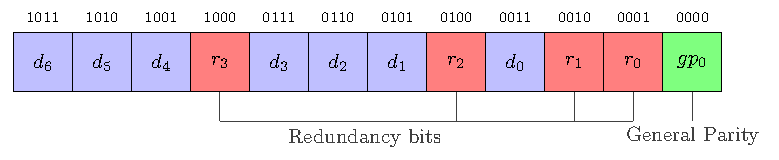
\includegraphics[page=1]{c5_countermeasures_dift/img/secded.pdf}
    \caption{Hamming Code -- SECDED (12,7) -- principle}
    \label{fig:secded_functionning}
\end{figure}

The fundamental principle behind SECDED compared to Hamming Codes is the addition of an extra bit to calculate the general parity $gp_0$ (Figure~\ref{fig:secded_functionning}). This extra bit works aside of the redundancy bits and helps calculate the parity of the whole message (redundancy bits and data bits). This bit helps detects two bits errors while being able to correct single-bit errors. The parity bit is generally placed at the beginning of the message at index \texttt{0}. As the most common Hamming Code is the (7,4), the most common SECDED code is the (8,4) with four bits of data, three redundancy bits and one parity bit.
Equation~\ref{equat:secded_encoder} presents the calculation of the different redundancy and parity bits for a message of seven data bits.
Figure~\ref{fig:secded_example} also represents the calculation of the general parity bit. This is the same message as for Hamming Codes (Figure~\ref{fig:hamming_code_example_1}), in the previous subsection, so the redundancy bits are already calculated. Figure~\ref{fig:secded_example_1} represents the initial message when all redundancy bits are calculated. If the message with the redundancy bits is equal to \texttt{0b10011100101}, the number of \texttt{1}s is even, then the general parity bit will be set to \texttt{0}, as depicted in Figure~\ref{fig:secded_example_2}.

\begin{equation} \label{equat:secded_encoder}
    \begin{split}
        r_{0}   = d_{0} \oplus d_{1} \oplus d_{3} \oplus d_{4} \oplus d_{6} \\
        r_{1}   = d_{0} \oplus d_{2} \oplus d_{3} \oplus d_{5} \oplus d_{6} \\
        r_{2}   = d_{1} \oplus d_{2} \oplus d_{3} \\
        r_{3}   = d_{4} \oplus d_{5} \oplus d_{6} \\
        gp_{0}  = d_{0} \oplus d_{1} \oplus d_{2} \oplus d_{3} \oplus d_{4} \oplus d_{5} \oplus d_{6} \oplus r_{0} \oplus r_{1} \oplus r_{2} \oplus r_{3}
    \end{split}
\end{equation}

\begin{figure}[ht]
    \centering
    \begin{subfigure}[b]{0.49\textwidth}
        \includegraphics[width=\textwidth, page=2]{c5_countermeasures_dift/img/secded.pdf}
        \caption{Initial message}
        \label{fig:secded_example_1}
    \end{subfigure}
    \hfill
    \begin{subfigure}[b]{0.49\textwidth}
        \includegraphics[width=\textwidth, page=4]{c5_countermeasures_dift/img/secded.pdf}
        \caption{Calculation of general parity bit $gp_0$}
        \label{fig:secded_example_2}
    \end{subfigure}
    \hfill
    \begin{subfigure}[b]{0.49\textwidth}
        \includegraphics[width=\textwidth, page=5]{c5_countermeasures_dift/img/secded.pdf}
        \caption{Final message}
        \label{fig:secded_example_3}
    \end{subfigure}
    \caption{SECDED (12,7) general parity bit calculation}
    \label{fig:secded_example}
\end{figure}

Figure~\ref{fig:secded_faulted_1bit} depicts the injection of a single-bit fault. The received message corresponds to the previous one (\texttt{0b100111001010}). A fault is injected in bit $d_3$ at position \texttt{0111} (seventh position).
The decoder calculation of redundancy bits are done at first in Figures~\ref{fig:secded_faulted_1bit_3}, \ref{fig:secded_faulted_1bit_4}, \ref{fig:secded_faulted_1bit_5}, and \ref{fig:secded_faulted_1bit_6} and then gives the syndrome \texttt{0b0111} for the seventh position which corresponds to the data bit $d_3$. This syndrome is correct. Now, the general parity bit is decoded from all bits of the message in Figure~\ref{fig:secded_faulted_1bit_7}. This time, the general parity bit is not correct (\texttt{1} instead of \texttt{0}). This new value means that a single fault occurred. Because the syndrome and the general parity bit are different of \texttt{0}.

\begin{figure}[ht]
    \centering
    \begin{subfigure}[b]{0.49\textwidth}
        \includegraphics[width=\textwidth, page=5]{c5_countermeasures_dift/img/secded.pdf}
        \caption{Initial message}
        \label{fig:secded_faulted_1bit_1}
    \end{subfigure}
    \hfill
    \begin{subfigure}[b]{0.49\textwidth}
        \includegraphics[width=\textwidth, page=6]{c5_countermeasures_dift/img/secded.pdf}
        \caption{Injection of a fault in bit $d_3$}
        \label{fig:secded_faulted_1bit_2}
    \end{subfigure}
    \hfill
    \begin{subfigure}[b]{0.49\textwidth}
        \includegraphics[width=\textwidth, page=7]{c5_countermeasures_dift/img/secded.pdf}
        \caption{Calculation of redundancy bit $r_0$}
        \label{fig:secded_faulted_1bit_3}
    \end{subfigure}
    \hfill
    \begin{subfigure}[b]{0.49\textwidth}
        \includegraphics[width=\textwidth, page=8]{c5_countermeasures_dift/img/secded.pdf}
        \caption{Calculation of redundancy bit $r_1$}
        \label{fig:secded_faulted_1bit_4}
    \end{subfigure}
    \hfill
    \begin{subfigure}[b]{0.49\textwidth}
        \includegraphics[width=\textwidth, page=9]{c5_countermeasures_dift/img/secded.pdf}
        \caption{Calculation of redundancy bit $r_2$}
        \label{fig:secded_faulted_1bit_5}
    \end{subfigure}
    \hfill
    \begin{subfigure}[b]{0.49\textwidth}
        \includegraphics[width=\textwidth, page=10]{c5_countermeasures_dift/img/secded.pdf}
        \caption{Calculation of redundancy bit $r_3$}
        \label{fig:secded_faulted_1bit_6}
    \end{subfigure}
    \hfill
    \begin{subfigure}[b]{0.49\textwidth}
        \includegraphics[width=\textwidth, page=11]{c5_countermeasures_dift/img/secded.pdf}
        \caption{Calculation of redundancy bit $gp_0$}
        \label{fig:secded_faulted_1bit_7}
    \end{subfigure}
    \caption{Example of a 1 bit fault with SECDED (12,7)}
    \label{fig:secded_faulted_1bit}
\end{figure}

Figure~\ref{fig:secded_faulted_2bits} depicts the injection of a double-bits fault. The received message is still the same (\texttt{0b100111001010}). A fault is injected in bit $d_3$ at position \texttt{0111} (seventh position) and another fault is injected in bit $d_0$ at position \texttt{0011}.
The decoder calculation of redundancy bits are done at first in Figures~\ref{fig:secded_faulted_2bits_3}, \ref{fig:secded_faulted_2bits_4}, \ref{fig:secded_faulted_2bits_5}, and \ref{fig:secded_faulted_2bits_6}, and gives the syndrome \texttt{0b0100} for the fourth position which corresponds to the redundancy bit $r_2$. This syndrome is incorrect and without the general parity bit, Hamming Code would correct the fourth bit, which would lead to the injection of a third fault in the message.
But thanks to SECDED, the general parity bit is decoded from all bits of the message in Figure~\ref{fig:secded_faulted_2bits_7}. This time, the general parity bit is correct (\texttt{0}). This value means that a double fault occurred because the parity did not change while the redundancy bits changed.

\begin{figure}[ht]
    \centering
    \begin{subfigure}[b]{0.49\textwidth}
        \includegraphics[width=\textwidth, page=5]{c5_countermeasures_dift/img/secded.pdf}
        \caption{Initial message}
        \label{fig:secded_faulted_2bits_1}
    \end{subfigure}
    \hfill
    \begin{subfigure}[b]{0.49\textwidth}
        \includegraphics[width=\textwidth, page=12]{c5_countermeasures_dift/img/secded.pdf}
        \caption{Injection of a fault in bit $d_3$ and bit $d_0$}
        \label{fig:secded_faulted_2bits_2}
    \end{subfigure}
    \hfill
    \begin{subfigure}[b]{0.49\textwidth}
        \includegraphics[width=\textwidth, page=13]{c5_countermeasures_dift/img/secded.pdf}
        \caption{Calculation of redundancy bit $r_0$}
        \label{fig:secded_faulted_2bits_3}
    \end{subfigure}
    \hfill
    \begin{subfigure}[b]{0.49\textwidth}
        \includegraphics[width=\textwidth, page=14]{c5_countermeasures_dift/img/secded.pdf}
        \caption{Calculation of redundancy bit $r_1$}
        \label{fig:secded_faulted_2bits_4}
    \end{subfigure}
    \hfill
    \begin{subfigure}[b]{0.49\textwidth}
        \includegraphics[width=\textwidth, page=15]{c5_countermeasures_dift/img/secded.pdf}
        \caption{Calculation of redundancy bit $r_2$}
        \label{fig:secded_faulted_2bits_5}
    \end{subfigure}
    \hfill
    \begin{subfigure}[b]{0.49\textwidth}
        \includegraphics[width=\textwidth, page=16]{c5_countermeasures_dift/img/secded.pdf}
        \caption{Calculation of redundancy bit $r_3$}
        \label{fig:secded_faulted_2bits_6}
    \end{subfigure}
    \hfill
    \begin{subfigure}[b]{0.49\textwidth}
        \includegraphics[width=\textwidth, page=17]{c5_countermeasures_dift/img/secded.pdf}
        \caption{Calculation of redundancy bit $gp_0$}
        \label{fig:secded_faulted_2bits_7}
    \end{subfigure}
    \caption{Example of two 1-bit faults with SECDED (12,7)}
    \label{fig:secded_faulted_2bits}
\end{figure}

\begin{table}[t]
    \centering
    \footnotesize
    \caption{Summarise of the three case for SECDED}
    \label{tab:sumup_secded}
    \begin{tabular}{@{}c|cc@{}}
        \toprule
        Fault Detection         & Redundancy Bits   & General Parity Bit \\\midrule
        No fault                & $\{r_0 - r_3\} = 0$ & $gp_0 = 0$        \\
        Single Error Correction & $\{r_0 - r_3\} \neq 0$                  & $gp_0 = 1$                   \\
        Double Errors Detection & $\{r_0 - r_3\} \neq 0$                  & $gp_0 = 0$                   \\
        \bottomrule
    \end{tabular}
\end{table}

To conclude on SECDED, this code allows correcting single-bit errors and detect double-bit errors in a message. It is a lightweight countermeasure, as it only adds a few redundancy bits and one general parity bit. When a fault occurs, there are three different possible cases represented in Table~\ref{tab:sumup_secded}. In the first case, the syndrome formed by the redundancy bits is equal to \texttt{0} and the general parity bit syndrome is also equal to \texttt{0}, in that case, nothing happened, the message is correct.
In the second case, if the syndrome formed by the redundancy bits is different from \texttt{0} and the general parity bit is equal to \texttt{1}, this means that an error has occurred and the syndrome of the redundancy bits will give its position to allow correction at the correct index.
The third case is represented by a redundancy bits syndrome different from \texttt{0} and a general parity bit equal to \texttt{0}, in that case, it means that a double bits error occurred. This time the error can not be corrected. The limitation of this code is achieved when a three bits error occurs.

%%%%%%%%%%%%%%%%%%%%%%%%%%%%%%
\subsection{Implementation: Minimisation of redundancy bits}

In order to implement SECDED, we used the same idea as the previous countermeasures: minimisation of redundancy bits. We used the same five groups as depicted in Table~\ref{tab:secded_group}. In total, we have to use \compute{25+6}{0} bits to protect our mechanism with SECDED against single-bit errors and double-bit errors.

\begin{table}[t]
    \centering
    \footnotesize
    \caption{DIFT-related protected registers -- SECDED}
    \label{tab:secded_group}
    \begin{tabular}{@{}cccccc@{}}
        \toprule
                & Protected register                                                                                & \begin{tabular}[c]{@{}c@{}}Number of\\ bits\end{tabular} & \begin{tabular}[c]{@{}c@{}}Number of\\ protected bits\end{tabular} & \begin{tabular}[c]{@{}c@{}}Number of\\ redundancy bits\end{tabular} & \begin{tabular}[c]{@{}c@{}}Number of\\ parity bits\end{tabular} \\ \midrule
        Group 1 & TCR                                                                                               & 32                                                       & 22                                                                 & 5                                                                   & 1                                                               \\
        Group 2 & TPR                                                                                               & 32                                                       & 22                                                                 & 5                                                                   & 1                                                               \\
        Group 3 & Register File (Tag)                                                                               & 32                                                       & 32                                                                 & 6                                                                   & 1                                                               \\
        Group 4 & Tag destination address                                                                           & 5                                                        & 5                                                                  & 4                                                                   & 1                                                               \\
        Group 5 & \begin{tabular}[c]{@{}c@{}}16×1-bit registers\\ 3×2-bit registers\\ 1×4-bit register\end{tabular} & 26                                                       & 26                                                                 & 5                                                                   & 1                                                               \\ \midrule
        Total   &                                                                                                   & 127                                                      & 107                                                                & 25                                                                  & 5                                                               \\
        \bottomrule
    \end{tabular}
\end{table}

Figure~\ref{fig:implementation_sd_1} and Figure~\ref{fig:implementation_sd_2} present the proposed implementations for SECDED. We do not integrate control signals for clarity in these figures. This is approximatively the same figures as for Hamming Code (Figure~\ref{fig:implementation_hc_1} and Figure~\ref{fig:implementation_hc_2}) but with the representation of the extra register that stores the general parity bit.

\begin{figure}[ht]
    \centering
    \includegraphics[page=4, width=\textwidth]{c5_countermeasures_dift/img/archi_contremesures.pdf}
    \caption{Implementation of SECDED}
    \label{fig:implementation_sd_1}
\end{figure}

\begin{figure}[ht]
    \centering
    \includegraphics[page=5, width=\textwidth]{c5_countermeasures_dift/img/archi_contremesures.pdf}
    \caption{Implementation of SECDED -- Register File Tag}
    \label{fig:implementation_sd_2}
\end{figure}

%%%%%%%%%%%%%%%%%%%%%%%%%%%%%%%%%%%%%%%%%%%%%%%%%%%%%%%%%%%%%%%%%%%%%%%%%%%%%%%%%%%%%%%%%%%%%%%
\section{Evaluation results}

This section presents logical fault injection simulation results considering our two fault models: \textit{single bit-flip in one register at a given clock cycle} and \textit{single bit-flip in two registers at two clock cycles}. For protected implementations, faults are injected into both DIFT-related and protection-related registers.

Table~\ref{tab:chap5_implementation} presents the results of the FPGA implementation using Vivado 2023.2, targeting the Xilinx Zynq-7000 of the Zedboard development board. It compares different protection mechanisms in terms of resource utilisation and maximum operating frequency. The table lists the number of Look-Up Tables (LUTs), the number of Flip-Flops (FFs), and the maximum achievable frequency for each protection scheme. The D-RI5CY mechanism serves as reference. The baseline version represents the processor without the DIFT protection, showing a reduction in both LUTs and FFs usage by 4.54\% and 5.31\%, respectively, while achieving a 3\% improvement in maximum frequency compared to the D-RI5CY.
Simple parity protection slightly increases LUTs usage by 1.45\%, with a negligible impact on FFs and no change in the maximum frequency. The Hamming Code protection implementation introduces more overhead, with a 5.38\% increase in LUTs and a 1.11\% increase in FFs, alongside a minor reduction in maximum frequency by 0.36\%.
SECDED, finally, introduces the most significant overhead, with an increase of 7.48\% in LUTs, and 1.33\% in FFs, and also decreases the maximum frequency by 0.95\%. This overhead is due to the combination of redundancy bits from Hamming Code and the general parity bit.
This comparison highlights the trade-offs between resource utilisation and performance across different protection mechanisms in FPGA implementations.

\begin{table}[t]
    \footnotesize
    \centering
    \caption{FPGA implementation results — Vivado 2023.2}
    \label{tab:chap5_implementation}
    \setlength{\tabcolsep}{3pt}
    \begin{tabular}{@{}c|ccc@{}}
        \toprule
        Protection    & Number of LUTs   & Number of FFs    & Maximum frequency                \\ \midrule
        Baseline      & 6,597 (-4.54\%) & 2,211 (-5.31\%) & \SI{49.1}{\mega\hertz} (3\%)     \\
        D-RI5CY       & 6,911 (0\%)     & 2,335 (0\%)     & \SI{47.6}{\mega\hertz} (0\%)     \\
        Simple parity & 7,011 (1.45\%)  & 2,337 (0.09\%)  & \SI{47.6}{\mega\hertz} (0\%)     \\
        Hamming Code  & 7,283 (5.38\%)  & 2,361 (1.11\%)  & \SI{47.4}{\mega\hertz} (-0.36\%) \\
        SECDED        & 7,428 (7.48\%)  & 2,366 (1.33\%)  & \SI{47.2}{\mega\hertz} (-0.95\%) \\
        \bottomrule
    \end{tabular}
\end{table}

Now, we will compare these protections in terms of security.
Regarding the "\textit{single bit-flip in one register at a given clock cycle}" fault model, Table~\ref{tab:chap5_results_single_bitflip} shows the results obtained for the three considered use cases with and without protections. It is worth noting that we never get any crashes since we target the DIFT-related registers only. These registers do not impact the control or instruction flow of the processor.
The results obtained without protection are from Chapter~\ref{chapter:dift_assessment}. We obtain \compute{12+29+10}{0} successes out of \compute{762+1016+508}{0} fault injection simulations with the D-RI5CY only.
Conversely, when employing simple parity protection, none of the \compute{792+1056+528}{0} simulations result in success, as each single-fault in this fault model is detected, achieving a 100\% detection rate. With simple parity, an error signal is generated, which can be intercepted by a software running in the system to handle the fault, potentially halting the application if necessary. In contrast, the Hamming Code protection corrects the fault within the same cycle it occurs, without providing any direct indication to the attacker. The results from the Hamming Code simulations also show 0 success, but this time 100\% of the faults are corrected. This ensures the application continues running as if no fault occurred. From the attacker’s perspective, the fault does not affect the system’s behaviour in any way.
Results obtained with SECDED show the same results as with Hamming Code, which is normal as this fault model inject only one fault per simulation.

\begin{table}[t]
    \scriptsize
    \centering
    \caption{Logical fault injection simulation campaigns results for single bit-flip in one register at a given clock cycle}
    \label{tab:chap5_results_single_bitflip}
    \setlength{\tabcolsep}{3pt}
    \begin{tabular}{@{}ccccccccccc@{}}
        \toprule
                                                          &               & Crash & Silent & Delay & Detection & \tableTwoLines{Detection \&}{Correction} & \tableTwoLines{Double Error}{Detection} & Success     & Total  & \tableTwoLines{Execution}{time} \\\midrule
        \multirow{4}{*}{\tableTwoLines{Buffer}{Overflow}} & No protection & 0     & 738    & 12    & --         & --                                        & --                                      & 12 (1.57\%) & 762    & 0:11                            \\
                                                          & Simple parity & 0     & 0      & 0     & 792       & --                                        & --                                      & 0           & 792    & 0:08                            \\
                                                          & Hamming Code  & 0     & 0      & 0     & --         & 912                                      & --                                      & 0           & 912    & 0:12                            \\
                                                          & SECDED        & 0     & 0      & 0     & --         & 942                                      & 0                                       & 0           & 942    & 0:03                            \\\midrule
        \multirow{4}{*}{\tableTwoLines{Format}{String}}   & No protection & 0     & 946    & 41    & --         & --                                        & --                                      & 29 (2.85\%) & 1,016  & 01:52                           \\
                                                          & Simple parity & 0     & 0      & 0     & 1,056     & --                                        & --                                      & 0           & 1,056  & 01:30                           \\
                                                          & Hamming Code  & 0     & 0      & 0     & --         & 1,216                                    & --                                      & 0           & 1,216  & 01:50                           \\
                                                          & SECDED        & 0     & 0      & 0     & --         & 1,256                                    & 0                                       & 0           & 1,256  & 01:55                           \\\midrule
        \multirow{4}{*}{\tableTwoLines{Compare}{Compute}} & No protection & 0     & 491    & 7     & -—         & --                                        & --                                      & 10 (1.97\%) & 508    & 0:02                            \\
                                                          & Simple parity & 0     & 0      & 0     & 528       & --                                        & --                                      & 0           & 528    & 0:02                            \\
                                                          & Hamming Code  & 0     & 0      & 0     & --         & 608                                      & --                                      & 0           & 608    & 0:03                            \\
                                                          & SECDED        & 0     & 0      & 0     & --         & 628                                      & 0                                       & 0           & 628    & 0:03                            \\\midrule
        Total                                             &               &       &        &       &           &                                          &                                         & 51          & 10,224 &                                 \\
        \bottomrule
    \end{tabular}
\end{table}

\begin{table}[t]
    \scriptsize
    \centering
    \caption{Logical fault injection simulation campaigns results for single bit-flip in two registers at two clock cycles}
    \label{tab:chap5_results_tempo}
    \setlength{\tabcolsep}{3pt}
    \begin{tabular}{@{}cccccccccc@{}}
        \toprule
                                                          &               & Crash & Silent  & Delay  & Detection & \tableTwoLines{Detection \&}{Correction} & Success         & Total     & \tableTwoLines{Execution}{time} \\\midrule
        \multirow{3}{*}{\tableTwoLines{Buffer}{Overflow}} & No protection & 0     & 238,633 & 1,143  & --         & --                                        & 2,159 (0.89\%)  & 241,935   & 42:12                           \\
                                                          & Simple parity & 0     & 0       & 0      & 261,360   & --                                        & 0               & 261,360   & 64:24                           \\
                                                          & Hamming Code  & 0     & 0       & 0      & --         & 346,560                                  & 0               & 346,560   & 66:48                           \\\midrule
        \multirow{3}{*}{\tableTwoLines{Format}{String}}   & No protection & 0     & 429,260 & 12,192 & --         & --                                        & 10,160 (2.25\%) & 451,612   & 544:52                          \\
                                                          & Simple parity & 0     & 0       & 0      & 487,872   & --                                        & 0               & 487,872   & 389:20                          \\
                                                          & Hamming Code  & 0     & 0       & 0      & --         & 646,912                                  & 0               & 646,912   & 1069:36                         \\\midrule
        \multirow{3}{*}{\tableTwoLines{Format}{String}}   & No protection & 0     & 90,432  & 2,795  & —         & —                                        & 3,547 (3.67\%)  & 96,774    & 12:42                           \\
                                                          & Simple parity & 0     & 0       & 0      & 104,544   & --                                        & 0               & 104,544   & 13:36                           \\
                                                          & Hamming Code  & 0     & 0       & 0      & --         & 138,624                                  & 0               & 138,624   & 20:32                           \\\midrule
        Total                                             &               &       &         &        &           &                                          & 15,866          & 2,776,193 &                                 \\
        \bottomrule
    \end{tabular}
\end{table}

Table~\ref{tab:chap5_results_tempo} presents the results obtained considering the "\textit{single bit-flip in two registers at two clock cycles}" fault model. We conducted \num{2776193} simulations to present the results of this new fault model. For each simulation, we choose two bits in the same register or two registers, and we choose two different cycles, then, we flip one bit at a first cycle and flip the other one at the other cycle. Since SECDED does not degrade the error correction performance of the Hamming Code, the correction and detection capabilities for the fault models under consideration remain identical to those of the Hamming Code. Therefore, the simulation results for this protection are not presented, as they would provide no additional insights or distinctions from the Hamming Code's performance.
Even if the current fault model injects two faults, Hamming Code is enough because it injects one fault in one cycle and another fault in the next cycle in the worst case. Hence, as Hamming Code corrects a fault within the same cycle of the fault, the two faults are twice a single fault from Hamming Code side.
However, Table~\ref{tab:chap5_results_tempo} shows that without any protection, \num{15866} fault injections among \compute{241935+451612+96774}{0} simulations (\compute{(15866/(241935+451612+96774))*100}{2}\%) lead to a successful attack in the three use cases, while no successes are reported from simple parity or Hamming Code. Each fault is corrected thanks to Hamming Code.


%%%%%%%%%%%%%%%%%%%%%%%%%%%%%%%%%%%%%%%%%%%%%%%%%%%%%%%%%%%%%%%%%%%%%%%%%%%%%%%%%%%%%%%%%%%%%%%
\section{Summary}
In this chapter, we presented three countermeasures in order to protect the DIFT mechanism against FIAs. For that, we considered two fault models: \textit{single bit-flip in one register at a given clock cycle} and \textit{single bit-flip in two registers at two clock cycles}. These fault models are used in real world FIAs.
The first countermeasure is based on parity code: simple parity and can be used to detect any errors. Thanks to this protection, we achieve a 100\% fault detection in our considered fault model, but with the downside of giving an indication to the attacker as we emit a signal which can be caught by a running software to halt the application.
On the other hand, we implemented a code-based protection: Hamming Code. This protection is limited to only detection and correction of an error in our case. We propose two implementations. The first implementation is used to protect a set of registers together. The second implementation targets the protection of the \textit{Register File Tag} with constraints such as the number of write ports available. Thanks to these implementations, we are able to handle 100\% of the injected fault and correct them without any direct indication to the attacker.
The third countermeasure is a Hamming Code with an additional parity bit, this protection is called SECDED for Single Error Correction, Double Error Detection. This protection has been implemented in the same exact way of Hamming Code, with the difference that each formed group comprises an additional general parity bit.
These three countermeasures give effective results against the two fault models we have considered, while on the other hand, they have a limited impact on system performance and surface area.

In the next chapter, we will evaluate these protections against more complex fault models such as multi bit-flip faults and explore different implementation strategies in order to have a more robust protection against a wider range of attacks and fault models.

%%%%%%%%%%%%%%%%%%%%%%%%%%%%%%%%%%%%%%%%%%%%%%%%%%%%%%%%%%%%%%%%%%%%%%%%%%%%%%%%%%%%%%%%%%%%%%%